\section{Auswertung}

\subsection{Pockelseffekt}

\subsubsection{Sinusmodulation}

Wir haben zwei getrennte Messreihen à ca. 15 Messpaaren aufgenommen. Ein Messpaar bestand daraus, sowohl bei positiver als auch bei negativer Spannung, den Wert der Gleichspannung zu finden, bei dem das Sinussignal mit doppelter Frequenz am besten sichtbar war.

Messreihe 1 wurde bei $2010 \pm 7 Hz$ Sinussignal aufgenommen, Messreihe 2 bei $1800 \pm 1 Hz$ bzw $1815 \pm 1 Hz$ aufgenommen. Der Frequenzgenerator zeigte bei Messreihe 1 einen Drift von ca. $2017 Hz$ auf $2003 Hz$, blieb aber bei Messreihe 2 bis auf kleine Schwankungen stabil. Die Frequenzänderung bei Messreihe 2 ergibt sich dadurch, dass wir die Messung für eine Mittagspause unterbrochen haben.

\begin{python}
from numpy import *

from numbers import *

def sinus_auswertung(u_plus, u_minus):
  u_halb = [u_plus[i] + u_minus[i] for i in range(len(u_plus))]

  print '\n'

  print r'\begin{tabular}{rrr} \toprule'
  print r' $U_+$ [V] & $U_i$ [V] & $U_{\lambda/2}$ [U] \\'
  print r' \midrule '

  for i in range(len(u_plus)):
    print r'{u_plus:> 5.1f}&{u_minus:> 5.1f}&{u_halb:> 5.1f}\\'.format(u_plus=u_plus[i], u_minus=-u_minus[i], u_halb=u_halb[i])

  print r'\bottomrule '
  print r'\end{tabular}'
  print '\n'
  print '\n'

  u_halb_a = array(u_halb)
  print '\n'
  #print r'Anzahl: {anzahl} \\'.format(anzahl = len(u_halb_a))
  #print r'Summe: {summe:.5f}\\'.format(summe = sum(u_halb_a))
  u_l2 = mean(u_halb_a)
  print r'$U_{\lambda/2}: % .5f$\\' %u_l2 
  s_u_l2 = std(u_halb_a)
  print r'$S_{U_{\lambda/2}}: %.5f$\\' % s_u_l2

  return u_l2, s_u_l2

  

u_plus_r  = [164.1, 162.4, 161.9, 161.9, 162.3, 158.2, 156.3, 156.0, 156.1, 156.6, 155.2, 154.7, 152.5, 151.2, 151.4, 150.3]
u_minus_r = [89.9, 90.6, 90.4, 90.2, 91.9, 92.9, 93.4, 93.3, 92.8, 93.4, 94.0, 94.6, 97.3, 98.3, 99.3, 99.4]

u_plus_s = [153.6, 155.6, 156.7, 156.7, 157.5, 155.3, 154.9, 156.0, 154.3, 153.7, 154.2, 154.8, 154.1, 154.8, 154.8]
u_minus_s = [99.9, 99.5, 98.6, 97.4, 98.6, 97.9, 100.4, 100.3, 104.0, 103.6, 103.8, 104.3, 104.6, 104.1, 104.3]  

u_l2_r, s_u_l2_r = sinus_auswertung(u_plus_r, u_minus_r)
u_l2_s, s_u_l2_s = sinus_auswertung(u_plus_s, u_minus_s)

print r'$$ r_{41} = \frac{\lambda d}{4l U_{\lambda / 2}} \left(  \sqrt{\frac{1}{2} \left( \frac{1}{n_1^2} + \frac{1}{n_3^2} \right)} \right)^3 $$'

print 'sowie den Fehler: '

print r'$$S_{r_{41}} = r_{41} \frac{S_{U_{\lambda/2}}}{U_{\lambda/2}} $$'

lmbd = 632.8e-9 #m
d = 2.4e-3 #m
l = 20.0e-3 #m
n1 = 1.522
n3 = 1.477

def r_41(lmbd, d, l, U, n1, n3):
  return d*lmbd/(4.0*l*U)*(0.5*(1/(n1**2) + 1/(n3**2)))**(1.5)

r_41_r = r_41(lmbd, d, l, u_l2_r, n1, n3)
s_r_41_r = r_41_r * s_u_l2_r / u_l2_r
r_41_s = r_41(lmbd, d, l, u_l2_s, n1, n3)
s_r_41_s = r_41_s * s_u_l2_s / u_l2_s

print r'$r_{41_r} = ', number_error_to_latex(r_41_r, s_r_41_r, 3, -12), r' m/V$\\'
print r'$r_{41_s} = ', number_error_to_latex(r_41_s, s_r_41_s, 3, -12), r' m/V$\\'


\end{python}

Zum Vergleich, der Literaturwert beträgt: $r_{41} = 23.4 pm/V$

\subsubsection{Sägezahnmodulation}

\begin{figure}[H]
 \centering
 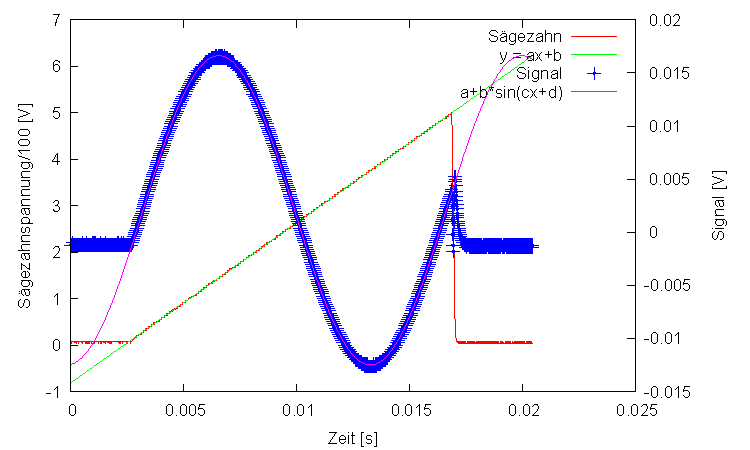
\includegraphics{messwerte/saegezahn/saegezahn_1.pdf}
 \caption{Sinusförmiges Signal als Reaktion auf eine Sägezahnspannung}
\end{figure}


Noch zu machen!


\subsection{Faradayeffekt}

Messung von $2\epsilon$:
$\alpha_1 = 8.4$

$\alpha_2 = 174,8$

\newcommand{\faradayDesc}{
Wir berechnen das Magnetfeld auf der Achse:

und integrieren darüber
$\int H dl$

Vergleich mit $ H = \frac{N I}{l} $

Berechnen die Verdetkonstante

$$ \alpha = l V H $$

Wir führen eine lineare Regression durch und erhalten die Steigung $a$ und den Achsenabschnitt $b$.

Es gilt $$ \alpha = V \int H(z) dz= V 2556 I = a I + b $$

Der Achsenabschnitt $b$ enthält den Offset bei der Winkelmessung und ist nicht weiter von Bedeutung.

Somit erhalten wir die Verdetkonstante aus $$ V = \frac{a}{2556} $$  

}

\begin{python}
from scipy import stats

from numbers import *

def auswertung_faraday(I, s_I, alpha, s_alpha):
  for i in range(len(alpha)):
    if alpha[i] > 100:
      alpha[i] = alpha[i]-180.0

  print '\n'

  print r'\begin{tabular}{rr} \toprule'
  print r' I [A] & $\alpha$ [$\circ$] \\'
  print r' \midrule '

  for i in range(len(I)):
    print r' {I:> 7.3g}  &  {alpha:> 7.3g} \\ '.format(I = I[i], alpha = alpha[i])

  print r'\bottomrule '
  print r'\end{tabular}'
  print '\n'
  print '\n'

  (a_s,b_s,r,tt,stderr)=stats.linregress(I, alpha)

  print r'Steigung: ' + repr(a_s)
  print r'Achsenab: ' + repr(b_s)

  return a_s, b_s


I_s = [-0.01, 0.5, 1.0, 1.5, 2.0, 2.5, 3.0, 3.5, 4.0, 4.47, +0.01, -0.5, -1.0, -1.5, -2.0, -2.5, -3.0, -3.5, -4.01, -4.50]
alpha_s = [0.50, 179.80, 178.05, 176.25, 175.42, 174.41, 173.10, 171.80, 170.48, 169.0, 0.55, 2.25, 3.40, 4.60, 5.85, 7.10, 8.40, 9.50, 10.80, 12.01]

I_r = [0.01, 0.5, 1.0, 1.5, 2.0, 2.5, 3.0, 3.5, 4.01, 4.52, -0.01, -0.51, -1.0, -1.5, -2.0, -2.49, -3.0, -3.5, -4.01, -4.53]
alpha_r = [0.35, 179.15, 177.9, 176.3, 175.0, 174.05, 172.65, 171.60, 170.25, 168.85, 0.40, 1.70, 3.10, 4.50, 5.55, 7.00, 8.25, 9.40, 10.80, 12.15]

s_I = 0.01
s_alpha = 0.4

a_s_s, b_s_s = auswertung_faraday(I_s, s_I, alpha_s, s_alpha)
a_s_r, b_s_r = auswertung_faraday(I_r, s_I, alpha_r, s_alpha)

print r'''\faradayDesc'''

print r'''
\begin{tabular}{rrr}
 \toprule
 Steigung $a$ & Achsenabschnitt $b$ & Verdetkonstante $V$ \\
 \midrule
''' + str(round(a_s_s, 3))+ r' & ' + str(round(b_s_s, 3)) + r' & ' + number_to_latex(a_s_s/2556, 5, -3) + r'''\\
''' + str(round(a_s_r, 3))+ r' & ' + str(round(b_s_r, 3)) + r' & ' + number_to_latex(a_s_r/2556, 5, -3) + r'''\\
 \bottomrule  
\end{tabular}
'''

\end{python}

